\documentclass[10pt, final, conference, letterpaper, onecolumn, oneside]{IEEEtran}
\usepackage{amsmath}
\usepackage{amssymb}
\usepackage{color}
\usepackage{tikz}
\usetikzlibrary{positioning}

\begin{document}

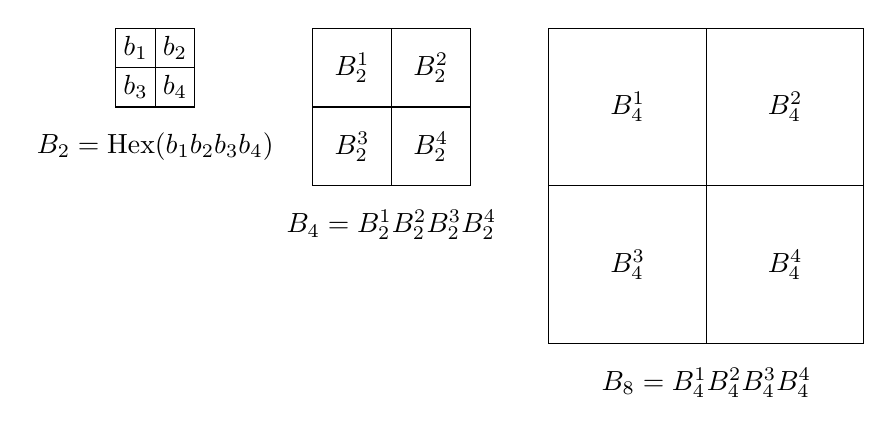
\begin{tikzpicture}[cell/.style={minimum size=0.5cm, draw, align=center, inner sep=0, outer sep=0},
  bigcell/.style={minimum size=1cm, draw, align=center, inner sep=0, outer sep=0},
  biggcell/.style={minimum size=2cm, draw, align=center, inner sep=0, outer sep=0},
  ]

  % First square with four cells
  \node[cell, anchor=north west] (b1) at (0,2) {$b_1$};
  \node[cell, right=0cm of b1] (b2) {$b_2$};
  \node[cell, below=0cm of b1] (b3) {$b_3$};
  \node[cell, right=0cm of b3] (b4) {$b_4$};

  % Text below the first square
  \node[below=0.5cm of b3.south east, anchor=center] {$B_2 = \text{Hex}(b_1b_2b_3b_4)$};

  % Second square to the right with sides twice the size
  \node[bigcell, anchor=north west, at=(b2.north east)] (B1) at (2.5,2) {$B_2^1$};
  \node[bigcell, right=0cm of B1] (B2) {$B_2^2$};
  \node[bigcell, below=0cm of B1] (B3) {$B_2^3$};
  \node[bigcell, right=0cm of B3] (B4) {$B_2^4$};

  % Text below the second square
  \node[below=0.5cm of B3.south east, anchor=center] {$B_4 = B_2^1B_2^2B_2^3B_2^4$};

  % Third square to the right with sides twice the size of second
  \node[biggcell, anchor=north west, at=(b2.north east)] (BB1) at (5.5,2) {$B_4^1$};
  \node[biggcell, right=0cm of BB1] (BB2) {$B_4^2$};
  \node[biggcell, below=0cm of BB1] (BB3) {$B_4^3$};
  \node[biggcell, right=0cm of BB3] (BB4) {$B_4^4$};

  % Text below the second square
  \node[below=0.5cm of BB3.south east, anchor=center] {$B_8 = B_4^1B_4^2B_4^3B_4^4$};

\end{tikzpicture}

\end{document}